\documentclass[]{standalone}

\usepackage{amsmath}
\usepackage{amsfonts}
\usepackage{amssymb}
\usepackage{graphicx}
\usepackage{tikz}
\usepackage{import}
\usepackage[subpreambles=true]{standalone}

\usepackage{tikz}
\usepackage{tikz-3dplot}

\usetikzlibrary{positioning}
\begin{document}

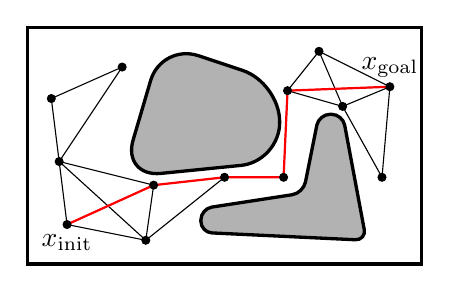
\begin{tikzpicture}[scale=1]

\useasboundingbox (0,0) rectangle (5,3);

\coordinate (init) at (0.5,0.5);
\coordinate (goal) at (4.6,2.25);
\coordinate (obs1) at (2.4,2.1);
\coordinate (obs2) at (3.7,0.65);
\coordinate (n0) at (0.4,1.3);
\coordinate (n1) at (1.2,2.5);
\coordinate (n2) at (1.5,0.3);
\coordinate (n3) at (4.5,1.1);
\coordinate (n4) at (1.6,1.0);
\coordinate (n5) at (4.0,2.0);
\coordinate (n6) at (3.3,2.2);
\coordinate (n7) at (3.25,1.1);
\coordinate (n8) at (2.5,1.1);
\coordinate (n9) at (0.3,2.1);
\coordinate (n10) at (3.7,2.7);

\path[draw] (n0) -- (n1);
\path[draw] (n0) -- (n2);
\path[draw] (n2) -- (n4);
\path[draw] (n8) -- (n4);
\path[draw] (n8) -- (n2);
\path[draw] (n7) -- (n8);
\path[draw] (n4) -- (n0);
\path[draw] (n3) -- (n5);
\path[draw] (n6) -- (n5);
\path[draw] (n7) -- (n6);
\path[draw] (n9) -- (n0);
\path[draw] (n9) -- (n1);
\path[draw] (n10) -- (n6);
\path[draw] (n10) -- (n5);

\path[draw] (init) -- (n0);
\path[draw] (init) -- (n2);
\path[draw] (init) -- (n4);

\path[draw] (goal) -- (n6);
\path[draw] (goal) -- (n10);
\path[draw] (goal) -- (n5);
\path[draw] (goal) -- (n3);

\path[draw=red, thick] (init) -- (n4) -- (n8) -- (n7) -- (n6) -- (goal);
    
\foreach \x in {0,...,10}
    \path[draw, fill] (n\x) circle (0.05);
    
\path[draw, very thick] (0,0) -- (5,0) -- (5,3) -- (0,3) -- cycle;
\path[draw, fill] (init) circle (0.05) node[below] {$x_\mathrm{init}$};
\path[draw, fill] (goal) circle (0.05) node[above] {$x_\mathrm{goal}$};

% \begin{scope}
%     \clip (0,0) rectangle (5,3);
%     \path[draw, thick, dashed, fill=gray, fill opacity=0.2] (n4) circle (1.3);
%     \path[draw, <->, thick] (n4) --  ++({cos(145)*1.3}, {sin(145)*1.3}) node [midway, shift={(-0.25,0)}] {$r$};
% \end{scope}

\path[draw, very thick, rounded corners=14pt, fill=black!30] (obs1) %node[shift={(-0.15,-0.25)}]{$\mathcal{C}_\mathrm{obs}$} 
    ++(-1.2,-1) -- ++(2,0.2) -- ++(0,1) -- ++(-1.5,0.5) -- cycle;
\path[draw, very thick, rounded corners=4pt, fill=black!30] (obs2) ++(-1.5,-0.25) -- ++(0,0.3) -- ++(1.3,0.2) -- ++(0.2,1) -- ++(0.3,0) -- ++(0.3,-1.6) -- cycle;

\end{tikzpicture}
\end{document}